% article.tex, a sample LaTeX file.
% Run LaTeX on this file twice for proper section numbers.
% A '%' causes LaTeX to ignore remaining text on the line

% Use the following line for draft mode (double spaced, single column)
\documentclass[preprint,pre,floats,aps,amsmath,amssymb]{revtex4}



% Use the following line for journal mode (single spaced, doublecolumn)
%\documentclass[twocolumn,pre,floats,aps,amsmath,amssymb]{revtex4}
\usepackage{graphicx}

\usepackage{bm}
\usepackage{enumerate}
\usepackage{wrapfig}
\usepackage{amsmath}
\usepackage{float}
\begin{document}


\title{scientific report: Jacobi method implementation on MS\_MPI 
}
\author{Ammar Ali Master Student}
\affiliation{Department Of Information Technology And Programming,Business Information System,ITMO University, Saint Petersburg  RUSSIA}
\date{\today}




\maketitle

\section{Introduction}
\label{sec:intro}
In this report, we will present the Jacobi method to solve linear equations. It is known that the Jacobi method has a complexity of O$[n^2]$ for each iteration and the number of iterations is related to the number of coefficients and to the required accuracy. We will use the Microsoft Messaging Passing Interface (MPI) library to implement the Jacobi method based on multi-threading instead of running on one thread. Then we will discuss how the multi-threading will affect the run-time.


\section{Discussion}
	\label{sec:Discussion}
\subsection{Jacobi method}
In numerical linear algebra, the Jacobi method is an iterative algorithm for determining the solutions of a strictly diagonally dominant system of linear equations. Each diagonal element is solved for, and an approximate value is plugged in. The process is then iterated until it converges. 
Let $Ax\; =\; b$ be a system of linear equations, where:\newline
$$A={\begin{bmatrix}a_{11}&a_{12}&\cdots &a_{1n}\\a_{21}&a_{22}&\cdots &a_{2n}\\\vdots &\vdots &\ddots &\vdots \\a_{n1}&a_{n2}&\cdots &a_{nn}\end{bmatrix}},\qquad \mathbf {x} ={\begin{bmatrix}x_{1}\\x_{2}\\\vdots \\x_{n}\end{bmatrix}},\qquad \mathbf {b} ={\begin{bmatrix}b_{1}\\b_{2}\\\vdots \\b_{n}\end{bmatrix}}.$$
If we decompose A into three matrices D,L,U where D is the diagonal component ,L the lower triangle and U the upper triangle.
Then we can obtain the solution iteratively according to the relation.
   $$x_{i}^{(k+1)}={\frac {1}{a_{ii}}}\left(b_{i}-\sum _{j\neq i}a_{ij}x_{j}^{(k)}\right),\quad i=1,2,\ldots ,n.$$
   A sufficient (but not necessary) condition for the method to converge is that the matrix A is strictly or irreducibly diagonally dominant. Strict row diagonal dominance means that for each row, the absolute value of the diagonal term is greater than the sum of absolute values of other terms:
   
   $${\displaystyle \left|a_{ii}\right|>\sum _{j\neq i}{\left|a_{ij}\right|}.}$$
   From the above it was shown that for each iteration we need to calculate a vector-matrix multiplication which needs O$[N^2]$ complexity. 
    
\section{Implementation}
\label{sec:implementation }
The idea is to split the matrix into parts and each thread will compute a part of the new vector in each iteration then we will gather the new vector from all threads and go to the second iteration. in each step it is also necessary to check the convergence "if the accuracy is more that a threshold value" to stop the infinite loop.
Also it is important to check the sufficient condition of the convergence before starting any iteration to avoid the non convergence situations which holds when the absolute value of a diagonal element is bigger than the summation of all other elements on the same row. and also this will be done using multi threading. We will use MS-MPI library to implement the algorithm.
To do that when we generate a random matrix we send data from one process to all other processes in a communicator. to do that we are using MPI\_Scatter\cite{MPI}.
\begin{figure}[h]
	\centering
	\caption{send data from one process to all other processes in a communicator}
	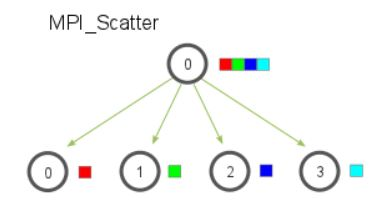
\includegraphics[scale=0.8]{1} 
	
\end{figure}
as well it was used when the vector is generated.
then to modify the new vector for each operation to calculate the distance and check for the convergence we need to gather the information form the processes.So, Given a set of elements distributed across all processes, MPI\_Allgather will gather all of the elements to all the processes\cite{MPI}. 
\begin{figure}[H]
	\centering
	\caption{ each process are gathered in order of their rank}
	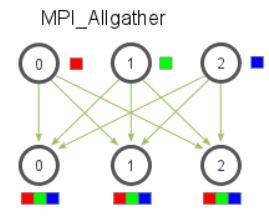
\includegraphics[scale=0.8]{2} 
	
\end{figure}



\section{Results}
\label{sec:results}

I generated $100000$ random numbers between 1 and 100 and run the code on a different number of threads as shown in fig(2). The best Running Time obtained when the number of threads equals 4 and for more threads, the run-time started to increase again.
Note:
tor run the code please using command window go to the directory of the debug in the project folder and type:\newline
mipexec -n 4 MPIfirst\newline
or specify any number of threads you want. Also maybe a conflict occurs because of using $ freopen$ to read from files.To solve this problem please add " \_CRT\_SECURE\_NO\_WARNINGS" to the $ Project\; Properties\; ->\; C/C++\;->\;Preprocessor\;->\;Preprocessor\;Definitions $. 

\newpage

I generated multiple matrices from dimensions of 100X100 to 2000X2000 increased by 200 so the testing matrices will have dimensions of the set (100,300,500,700 ..). The number of iterations initialized to be 300 with Error permission EPS equals to $10^{-6}$. But it was shown that all matrices will converge after maximum 67 iterations as long as it is a diagonal dominated matrix.
The testing matrices computed using different number of threads between 1 and 8 (Max of my laptop).And it showed the best number of threads to be used is different according to the size of matrices.
 \begin{figure}[H]

 	\caption{run-time according to number of used threads for different matrix dimensions}
 	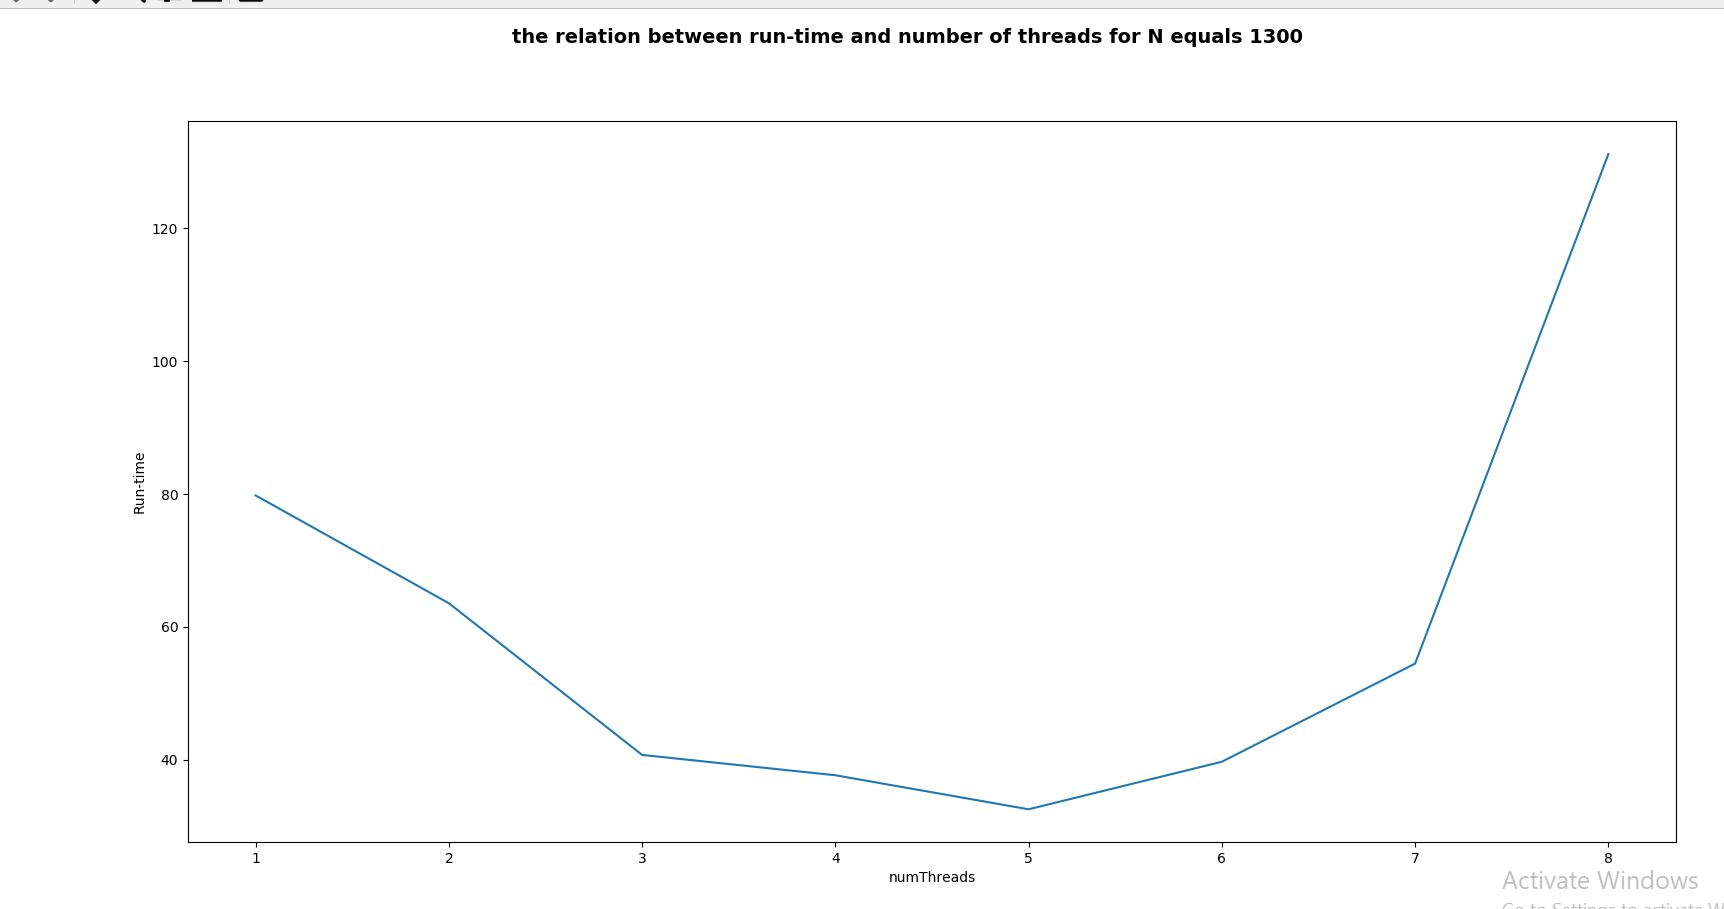
\includegraphics[scale=0.25]{3}
 	 	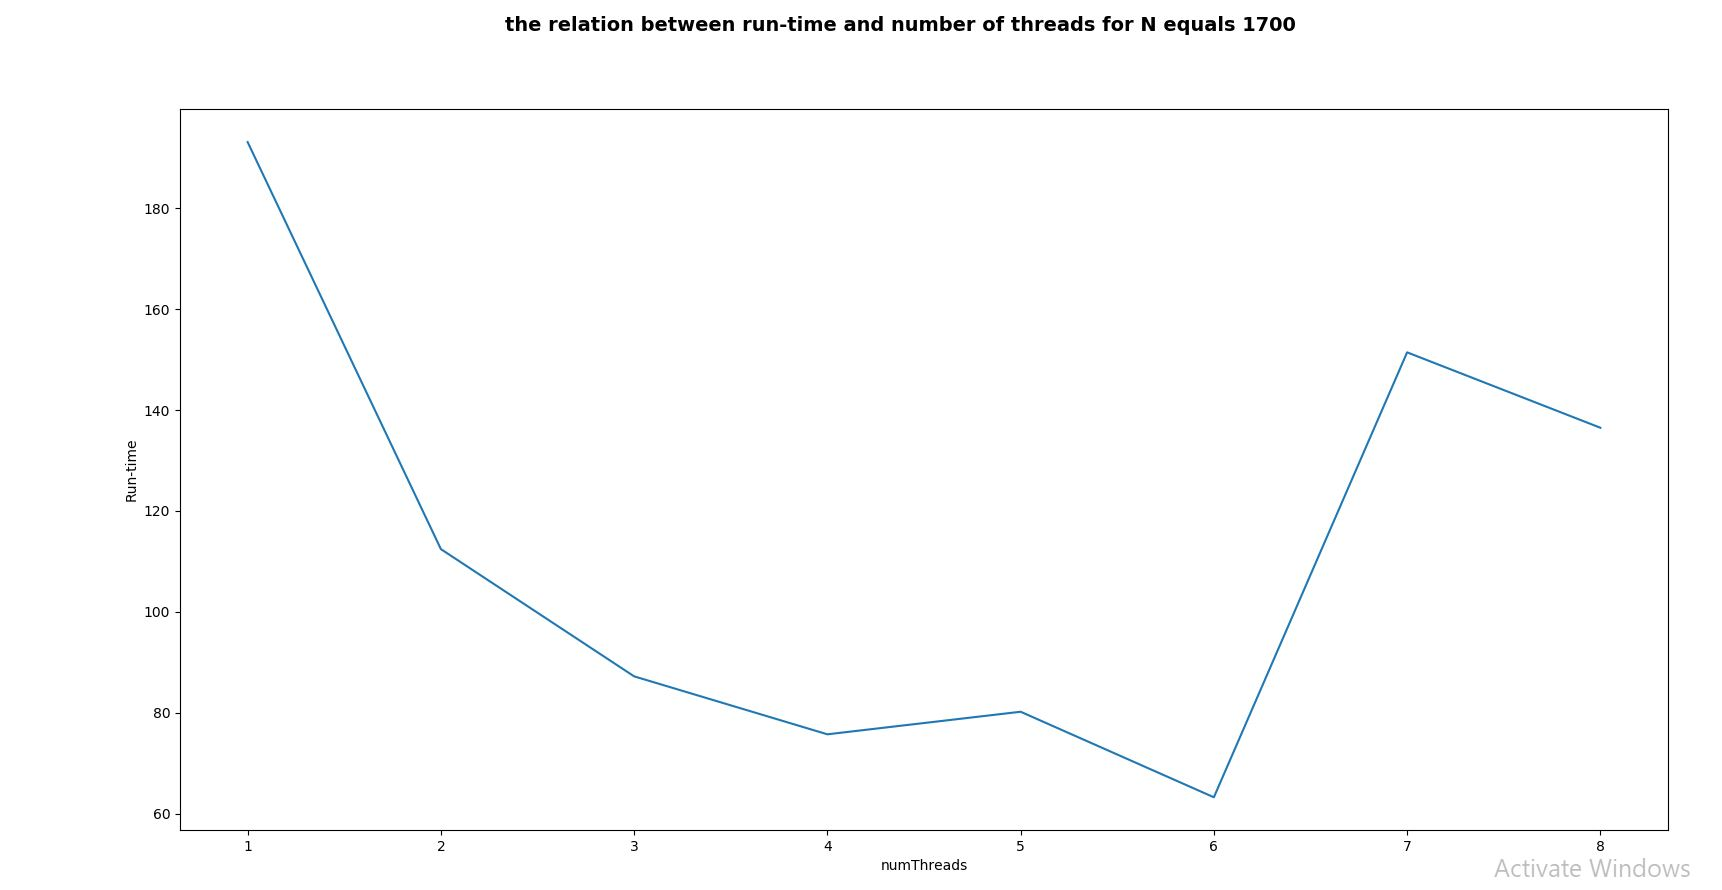
\includegraphics[scale=0.25]{4}
 	 	 	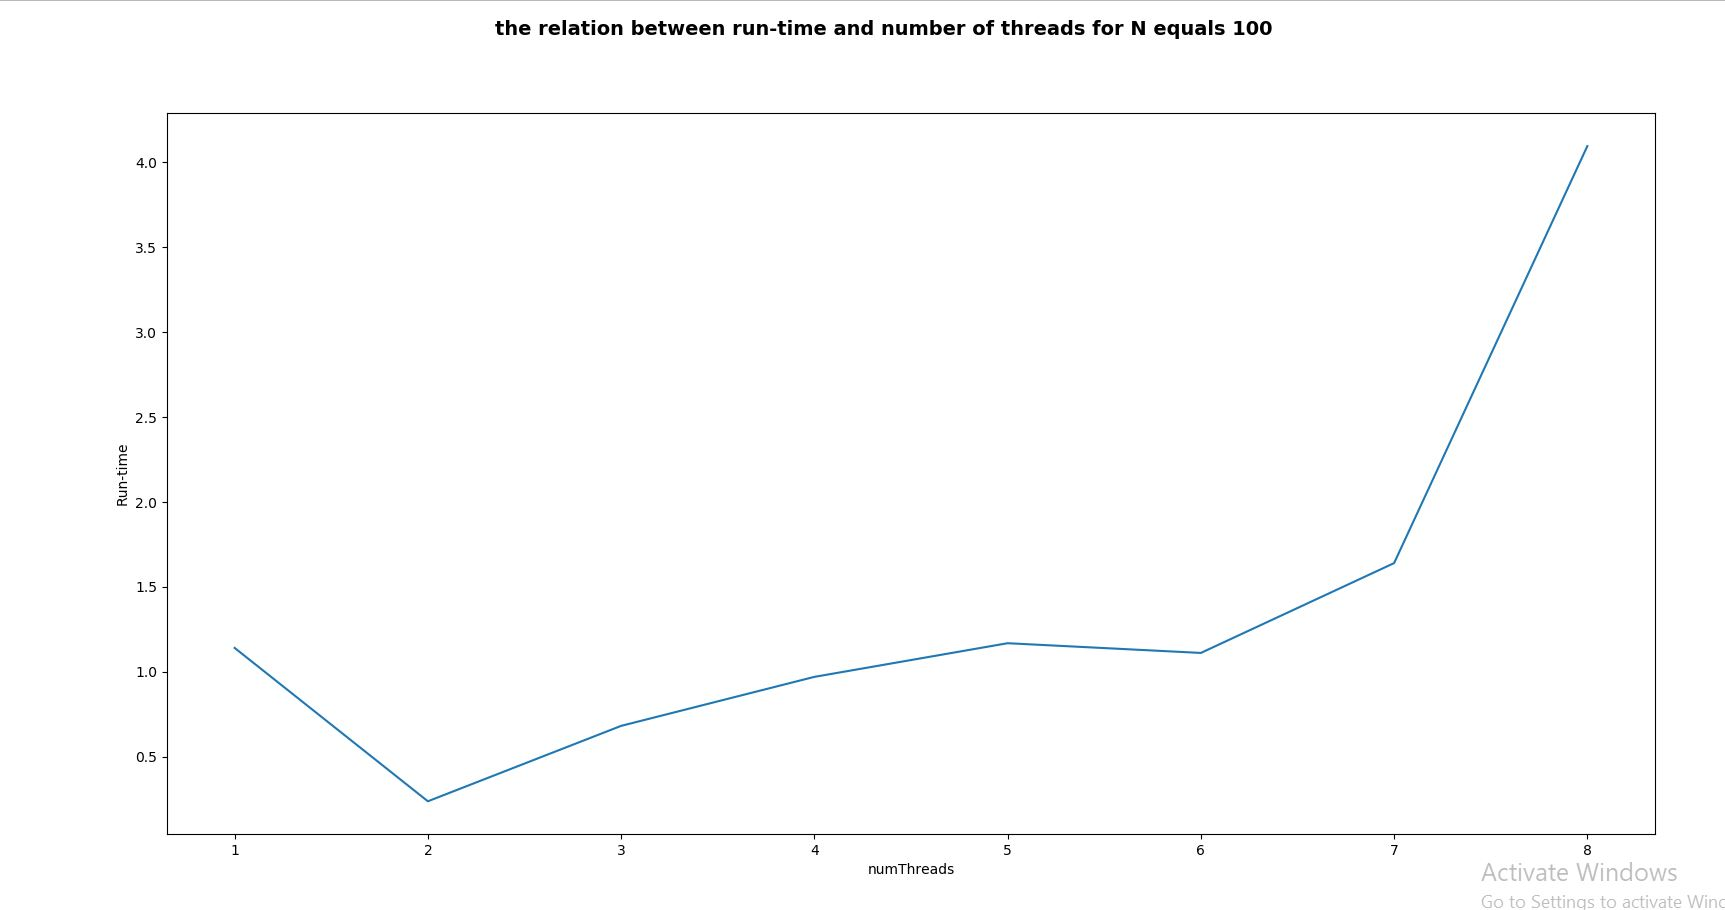
\includegraphics[scale=0.25]{5}
 	
 \end{figure}
As shown in the figures, the optimized number of threads related to the matrix dimensions. For small dimensions as 100 it shwoed that two threads will give the best running time by decreasing it more than the half in comparison with running on one thread.
for a matrix dimension of 1700 the best performance was using 6 threads where the running time divided by three.`
To see all figures please run the provided script. 
\begin{thebibliography}{9}
	\section{Reference}
	\bibitem{MPI} 
 
	[\textit{https://mpitutorial.com/tutorials/mpi-scatter-gather-and-allgather/ }]. 

	

	
\end{thebibliography}
\appendix*



\end{document}             % End of document.

